% ============================================================
%  TreeFlowNet — Architecture Diagram
%  Style reference: HoVer-Net (Graham et al. 2019),
%                   EmbedSeg (Lalit et al. 2022),
%                   FG-TreeSeg (Chen et al. 2026)
%  IEEE TGRS / ISPRS P&RS format
%  Engine: pdflatex + TikZ
% ============================================================
\documentclass[tikz, border=6pt]{standalone}

\usepackage{tikz}
\usepackage{amsmath, amssymb}
\usepackage{xcolor}

\usetikzlibrary{
  arrows.meta, calc, fit, positioning,
  shapes.geometric, backgrounds,
  decorations.pathreplacing, decorations.markings
}

% ── Color scheme (restrained, like HoVer-Net / EmbedSeg) ──
% At most 4 hues: charcoal, teal, amber, burgundy
\definecolor{cBlue}{HTML}{2C5F8A}      % backbone / encoder
\definecolor{cTeal}{HTML}{217A6E}      % FPN / neck
\definecolor{cGreen}{HTML}{2D6A4F}     % flow head
\definecolor{cPurple}{HTML}{5C3D8F}    % SDT head
\definecolor{cOrange}{HTML}{B5451B}    % centroid head
\definecolor{cBrown}{HTML}{7B4F2E}     % canopy head
\definecolor{cSlate}{HTML}{2C3E50}     % decoder
\definecolor{cDark}{HTML}{1A252F}      % outputs
\definecolor{cBg}{HTML}{F4F4F2}        % panel background
\definecolor{cLine}{HTML}{999999}      % light connector
\definecolor{cBrace}{HTML}{555555}     % brace / bracket
\definecolor{cLoss}{HTML}{8B1A1A}      % loss text

% ── Shared styles ──────────────────────────────────────────
\tikzset{
  % Standard module box
  mbox/.style 2 args={
    rectangle, rounded corners=3pt,
    minimum width=#1, minimum height=#2,
    fill=##1, draw=##1!70!black, line width=0.6pt,
    text=white, font=\small\sffamily, align=center,
  },
  % Section background panel (light gray, thin border)
  panel/.style={
    rectangle, rounded corners=4pt,
    fill=cBg, draw=cBg!60!black, line width=0.4pt,
    inner sep=6pt,
  },
  % Thin connector arrow
  arr/.style={
    -Stealth, line width=0.8pt, color=cBrace,
    shorten >=1pt, shorten <=1pt,
  },
  % Skip / residual (dashed)
  skip/.style={
    -Stealth, dashed, line width=0.55pt, color=cLine,
    shorten >=1pt, shorten <=1pt,
  },
  % Loss label
  loss/.style={
    font=\tiny\sffamily\itshape, text=cLoss,
    align=center,
  },
  % Section title above panel
  ptitle/.style={
    font=\scriptsize\sffamily\bfseries, text=cBrace,
    above, inner sep=2pt,
  },
}

\begin{document}
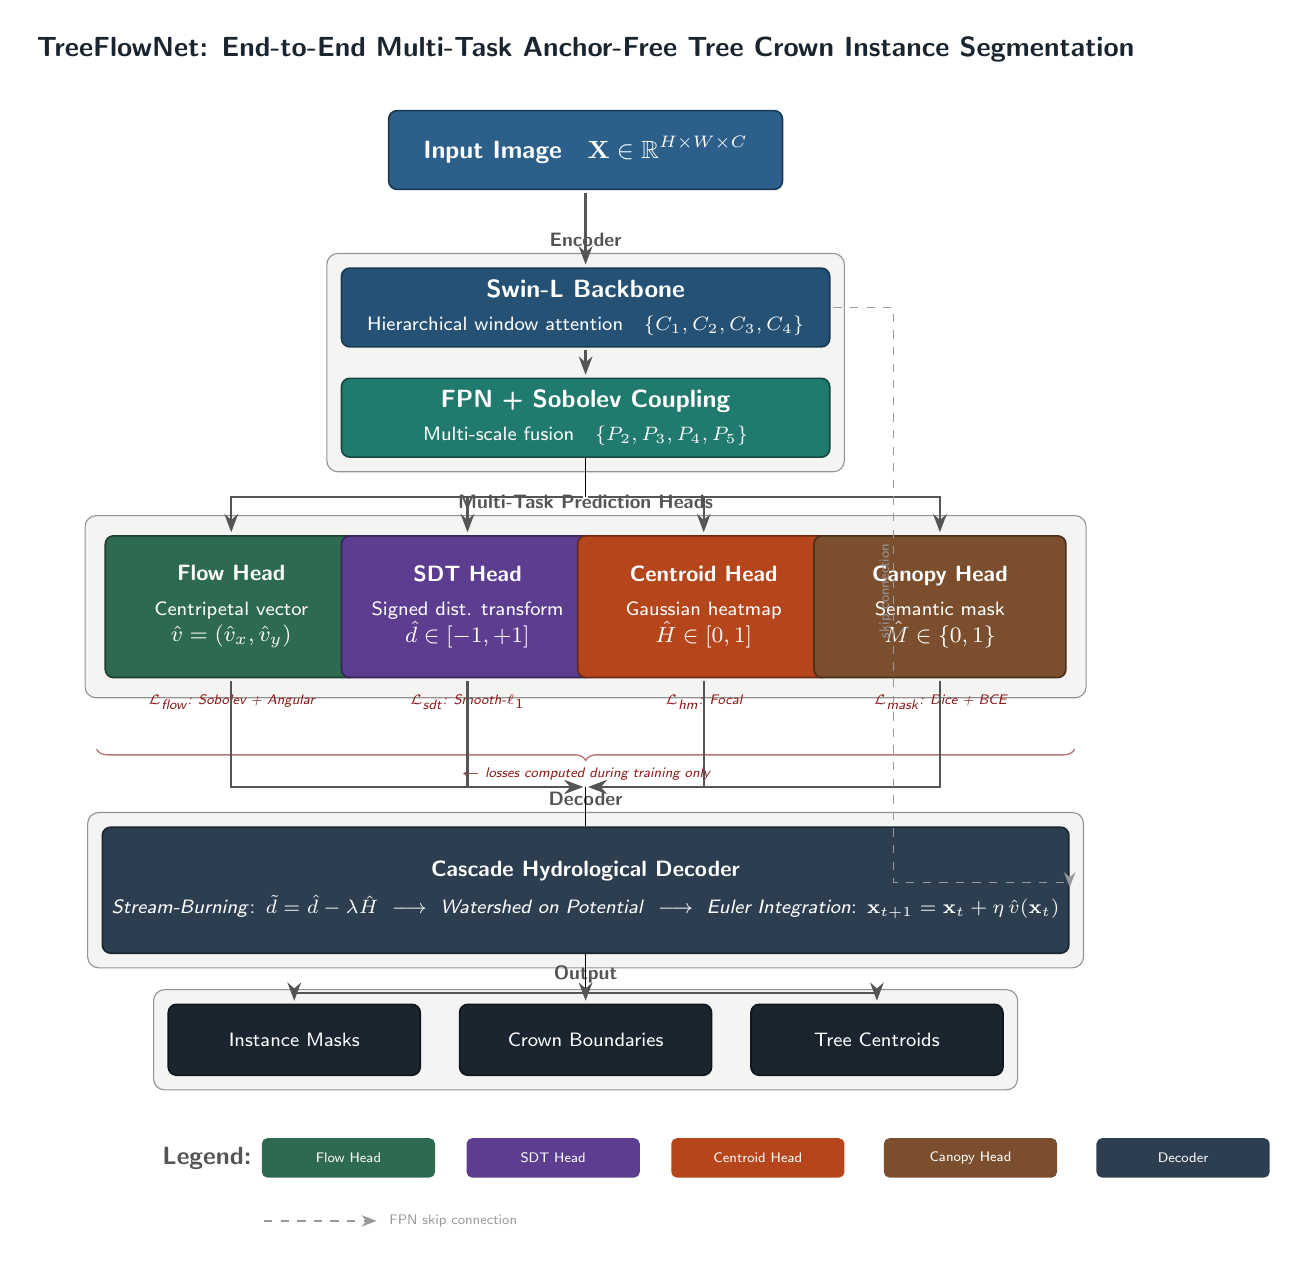
\begin{tikzpicture}[x=1mm, y=1mm, node distance=0mm]

% ═══════════════════════════════════════════════════════════
%  LAYOUT: vertical pipeline, 6 rows
%  Row positions (y of box center):
%    input    y=0
%    backbone y=-20
%    fpn      y=-36
%    heads    y=-60   (4 columns: x = -45, -15, +15, +45)
%    decoder  y=-90
%    outputs  y=-112  (3 columns)
% ═══════════════════════════════════════════════════════════

%────────────────────────────────────────────────────
% (1) INPUT
%────────────────────────────────────────────────────
\node[
  rectangle, rounded corners=3pt,
  minimum width=50mm, minimum height=10mm,
  fill=cBlue, draw=cBlue!60!black, line width=0.6pt,
  text=white, font=\small\sffamily, align=center,
] (inp) at (0,0)
  {\textbf{Input Image}\quad $\mathbf{X}\in\mathbb{R}^{H\times W\times C}$};

%────────────────────────────────────────────────────
% (2) ENCODER GROUP
%────────────────────────────────────────────────────
\node[
  rectangle, rounded corners=3pt,
  minimum width=62mm, minimum height=10mm,
  fill=cBlue!85!black, draw=cBlue!60!black, line width=0.6pt,
  text=white, font=\small\sffamily, align=center,
] (bb) at (0,-20)
  {\textbf{Swin-L Backbone}\\[1pt]
   \scriptsize Hierarchical window attention\quad $\{C_1,C_2,C_3,C_4\}$};

\node[
  rectangle, rounded corners=3pt,
  minimum width=62mm, minimum height=10mm,
  fill=cTeal, draw=cTeal!60!black, line width=0.6pt,
  text=white, font=\small\sffamily, align=center,
] (fpn) at (0,-34)
  {\textbf{FPN + Sobolev Coupling}\\[1pt]
   \scriptsize Multi-scale fusion\quad $\{P_2,P_3,P_4,P_5\}$};

% panel around encoder
\begin{scope}[on background layer]
  \node[panel, fit=(bb)(fpn), inner sep=5pt] (encpanel) {};
\end{scope}
\node[ptitle] at (encpanel.north) {Encoder};

%────────────────────────────────────────────────────
% (3) FOUR PREDICTION HEADS
%────────────────────────────────────────────────────

% Head boxes (y center = -58)
\node[
  rectangle, rounded corners=3pt,
  minimum width=32mm, minimum height=18mm,
  fill=cGreen, draw=cGreen!60!black, line width=0.6pt,
  text=white, font=\footnotesize\sffamily, align=center,
] (hf) at (-45,-58)
  {\textbf{Flow Head}\\[3pt]
   \scriptsize Centripetal vector\\
   $\hat{v}=(\hat{v}_x,\hat{v}_y)$};

\node[
  rectangle, rounded corners=3pt,
  minimum width=32mm, minimum height=18mm,
  fill=cPurple, draw=cPurple!60!black, line width=0.6pt,
  text=white, font=\footnotesize\sffamily, align=center,
] (hs) at (-15,-58)
  {\textbf{SDT Head}\\[3pt]
   \scriptsize Signed dist. transform\\
   $\hat{d}\in[-1,{+}1]$};

\node[
  rectangle, rounded corners=3pt,
  minimum width=32mm, minimum height=18mm,
  fill=cOrange, draw=cOrange!60!black, line width=0.6pt,
  text=white, font=\footnotesize\sffamily, align=center,
] (hh) at (15,-58)
  {\textbf{Centroid Head}\\[3pt]
   \scriptsize Gaussian heatmap\\
   $\hat{H}\in[0,1]$};

\node[
  rectangle, rounded corners=3pt,
  minimum width=32mm, minimum height=18mm,
  fill=cBrown, draw=cBrown!60!black, line width=0.6pt,
  text=white, font=\footnotesize\sffamily, align=center,
] (hm) at (45,-58)
  {\textbf{Canopy Head}\\[3pt]
   \scriptsize Semantic mask\\
   $\hat{M}\in\{0,1\}$};

% Loss labels below each head
\node[loss] at ($(hf.south)+(0,-3mm)$)
  {$\mathcal{L}_{\text{flow}}$: Sobolev + Angular};
\node[loss] at ($(hs.south)+(0,-3mm)$)
  {$\mathcal{L}_{\text{sdt}}$: Smooth-$\ell_1$};
\node[loss] at ($(hh.south)+(0,-3mm)$)
  {$\mathcal{L}_{\text{hm}}$: Focal};
\node[loss] at ($(hm.south)+(0,-3mm)$)
  {$\mathcal{L}_{\text{mask}}$: Dice + BCE};

% Panel around heads
\begin{scope}[on background layer]
  \node[panel, fit=(hf)(hs)(hh)(hm), inner sep=7pt] (hdpanel) {};
\end{scope}
\node[ptitle] at (hdpanel.north) {Multi-Task Prediction Heads};

% Training-only brace
\draw[decorate, decoration={brace, amplitude=4pt, mirror},
      color=cLoss!60, line width=0.5pt]
  ($(hf.south west)+(-1mm,-9mm)$) -- ($(hm.south east)+(1mm,-9mm)$)
  node[midway, below=3pt, font=\tiny\sffamily\itshape, text=cLoss]
  {$\leftarrow$ losses computed during training only};

%────────────────────────────────────────────────────
% (4) CASCADE DECODER
%────────────────────────────────────────────────────
\node[
  rectangle, rounded corners=3pt,
  minimum width=108mm, minimum height=16mm,
  fill=cSlate, draw=cSlate!60!black, line width=0.6pt,
  text=white, font=\footnotesize\sffamily, align=center,
] (dec) at (0,-94)
  {\textbf{Cascade Hydrological Decoder}\\[4pt]
   \scriptsize
   \textit{Stream-Burning}:\enspace
   $\tilde{d}=\hat{d}-\lambda\hat{H}$
   $\;\longrightarrow\;$
   \textit{Watershed on Potential}
   $\;\longrightarrow\;$
   \textit{Euler Integration}:\enspace
   $\mathbf{x}_{t+1}=\mathbf{x}_t+\eta\,\hat{v}(\mathbf{x}_t)$};

\begin{scope}[on background layer]
  \node[panel, fit=(dec), inner sep=5pt] (decpanel) {};
\end{scope}
\node[ptitle] at (decpanel.north) {Decoder};

%────────────────────────────────────────────────────
% (5) OUTPUTS
%────────────────────────────────────────────────────
\node[
  rectangle, rounded corners=3pt,
  minimum width=32mm, minimum height=9mm,
  fill=cDark, draw=cDark!60!black, line width=0.6pt,
  text=white, font=\scriptsize\sffamily, align=center,
] (oi) at (-37,-113) {Instance Masks};

\node[
  rectangle, rounded corners=3pt,
  minimum width=32mm, minimum height=9mm,
  fill=cDark, draw=cDark!60!black, line width=0.6pt,
  text=white, font=\scriptsize\sffamily, align=center,
] (ob) at (0,-113) {Crown Boundaries};

\node[
  rectangle, rounded corners=3pt,
  minimum width=32mm, minimum height=9mm,
  fill=cDark, draw=cDark!60!black, line width=0.6pt,
  text=white, font=\scriptsize\sffamily, align=center,
] (oc) at (37,-113) {Tree Centroids};

\begin{scope}[on background layer]
  \node[panel, fit=(oi)(ob)(oc), inner sep=5pt] (outpanel) {};
\end{scope}
\node[ptitle] at (outpanel.north) {Output};

%────────────────────────────────────────────────────
% ARROWS
%────────────────────────────────────────────────────

% Input → Backbone
\draw[arr] (inp.south) -- (bb.north);

% Backbone → FPN
\draw[arr] (bb.south) -- (fpn.north);

% FPN → Heads (fan-out via mid-point)
\coordinate (fanout) at ($(fpn.south)+(0,-5mm)$);
\draw (fpn.south) -- (fanout);
\draw[arr] (fanout) -| (hf.north);
\draw[arr] (fanout) -| (hs.north);
\draw[arr] (fanout) -| (hh.north);
\draw[arr] (fanout) -| (hm.north);

% Heads → Decoder (fan-in)
\coordinate (fanin) at ($(dec.north)+(0,5mm)$);
\draw (fanin) -- (dec.north);
\draw[arr] (hf.south) |- (fanin);
\draw[arr] (hs.south) |- (fanin);
\draw[arr] (hh.south) |- (fanin);
\draw[arr] (hm.south) |- (fanin);

% Decoder → Outputs (fan-out)
\coordinate (fano2) at ($(dec.south)+(0,-5mm)$);
\draw (dec.south) -- (fano2);
\draw[arr] (fano2) -| (oi.north);
\draw[arr] (fano2) -- (ob.north);
\draw[arr] (fano2) -| (oc.north);

% Skip connection: Backbone → Decoder (right side, dashed)
\draw[skip]
  (bb.east) -- ++(8mm,0) coordinate (skA)
  -- ($(skA)+(0,-73mm)$) coordinate (skB)
  -- (dec.east |- skB)
  -- (dec.east);
\node[font=\tiny\sffamily, text=cLine, rotate=90, anchor=south]
  at ($(skA)+(1mm,-36mm)$) {skip connection};

%────────────────────────────────────────────────────
% FIGURE TITLE
%────────────────────────────────────────────────────
\node[
  font=\normalsize\sffamily\bfseries, text=cDark,
  anchor=south, align=center,
] at (0,10) {TreeFlowNet: End-to-End Multi-Task Anchor-Free Tree Crown Instance Segmentation};

%────────────────────────────────────────────────────
% LEGEND (bottom)
%────────────────────────────────────────────────────
\node[font=\small\sffamily\bfseries, text=cBrace, anchor=west]
  (leg0) at (-55,-128) {Legend:};

% colored pills
\foreach \col/\lbl/\xo in {
  cGreen/{Flow Head}/0,
  cPurple/{SDT Head}/26,
  cOrange/{Centroid Head}/52,
  cBrown/{Canopy Head}/79,
  cSlate/{Decoder}/106}
{
  \node[
    rectangle, rounded corners=2pt,
    minimum width=22mm, minimum height=5mm,
    fill=\col, text=white, font=\tiny\sffamily,
    anchor=west,
  ] at ($(leg0.east)+(\xo mm, 0)$) {\lbl};
}

% dashed legend
\draw[skip] ($(leg0.east)+(0,-8mm)$) -- ++(15mm,0)
  node[right, font=\tiny\sffamily, text=cLine] {FPN skip connection};

\end{tikzpicture}
\end{document}
